%
% Copyright (c) 2011-2012, fortiss GmbH.
% Licensed under the Apache License, Version 2.0.
% 
% Use, modification and distribution are subject to the terms specified
% in the accompanying license file LICENSE.txt located at the root directory
% of this software distribution. A copy is available at
% http://chromosome.fortiss.org/.
%
% This file is part of CHROMOSOME.
%
% $Id$
%
% Author:
%         Michael Geisinger <geisinger@fortiss.org>
%

\section{Installing CMake}
\label{appx:install_cmake}

Follow these steps to install CMake:

\begin{enumerate}
	\item Point your faviorite browser to \url{http://cmake.org/cmake/resources/software.html}
		and click on the link corresponding to the Windows installer
		(compare Figure~\ref{fig:setup_cmake_download}).

\begin{figure}[htbp]
	\centering
	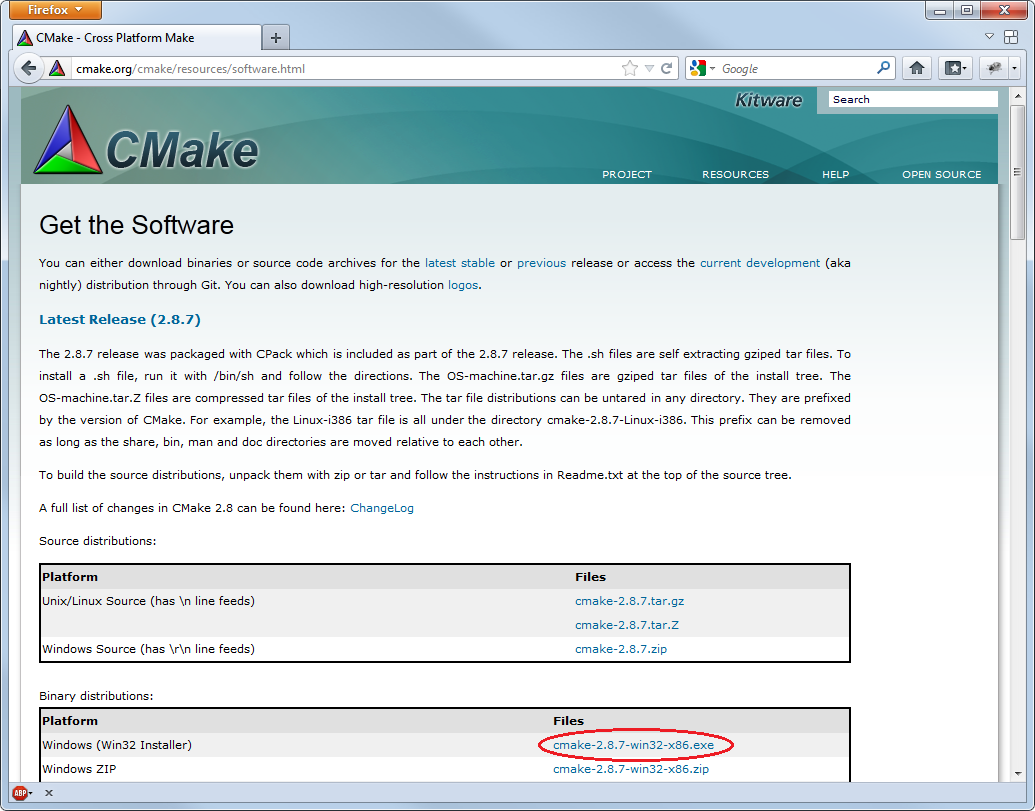
\includegraphics[scale=0.4]{figures/PNG/setup_cmake_download_edited.png}
	\caption{Selecting CMake for download, highlighted in red the download link.}
	\label{fig:setup_cmake_download}
\end{figure}

	\item After downloading the setup, launch it. Follow the instructions on the screen.
		When you get prompted whether to add CMake to the system PATH, you may choose to \emph{not} add it
		(compare Figure~\ref{fig:setup_cmake_path}).
		\xme does not require CMake to be on the system search path.

\begin{figure}[htbp]
	\centering
	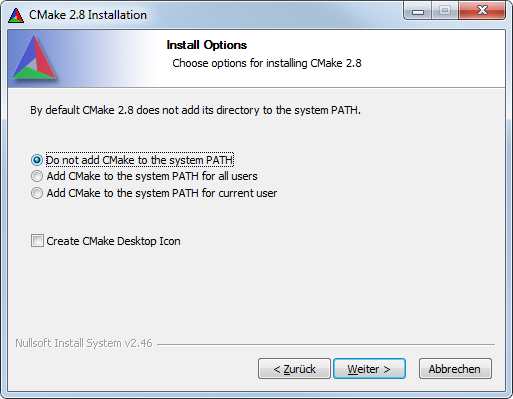
\includegraphics[scale=0.75]{figures/PNG/setup_cmake_path.png}
	\caption{CMake system PATH options.}
	\label{fig:setup_cmake_path}
\end{figure}

\end{enumerate}
